\begin{frame}{Future addition: $x y$ information}


\begin{columns}[c]
  \column{.5\textwidth}

  \begin{block}{Adding $x y$ information}
       \begin{itemize}
           \item Point of maximum $z$ in $x y$ available
           \item Extra information: sharp discontinuities between PVs
           \item Need iterative approach or ``reduced importance''
       \end{itemize}
  \end{block}

 \begin{block}{What about a full 2D kernel?}
      \begin{itemize}
          \item Not needed for LHCb currently (large $x y$, ``low'' $z$ overlap)
          \item Might be useful for other detectors!
      \end{itemize}
 \end{block}

 \column{.5\textwidth}
 \begin{center}
     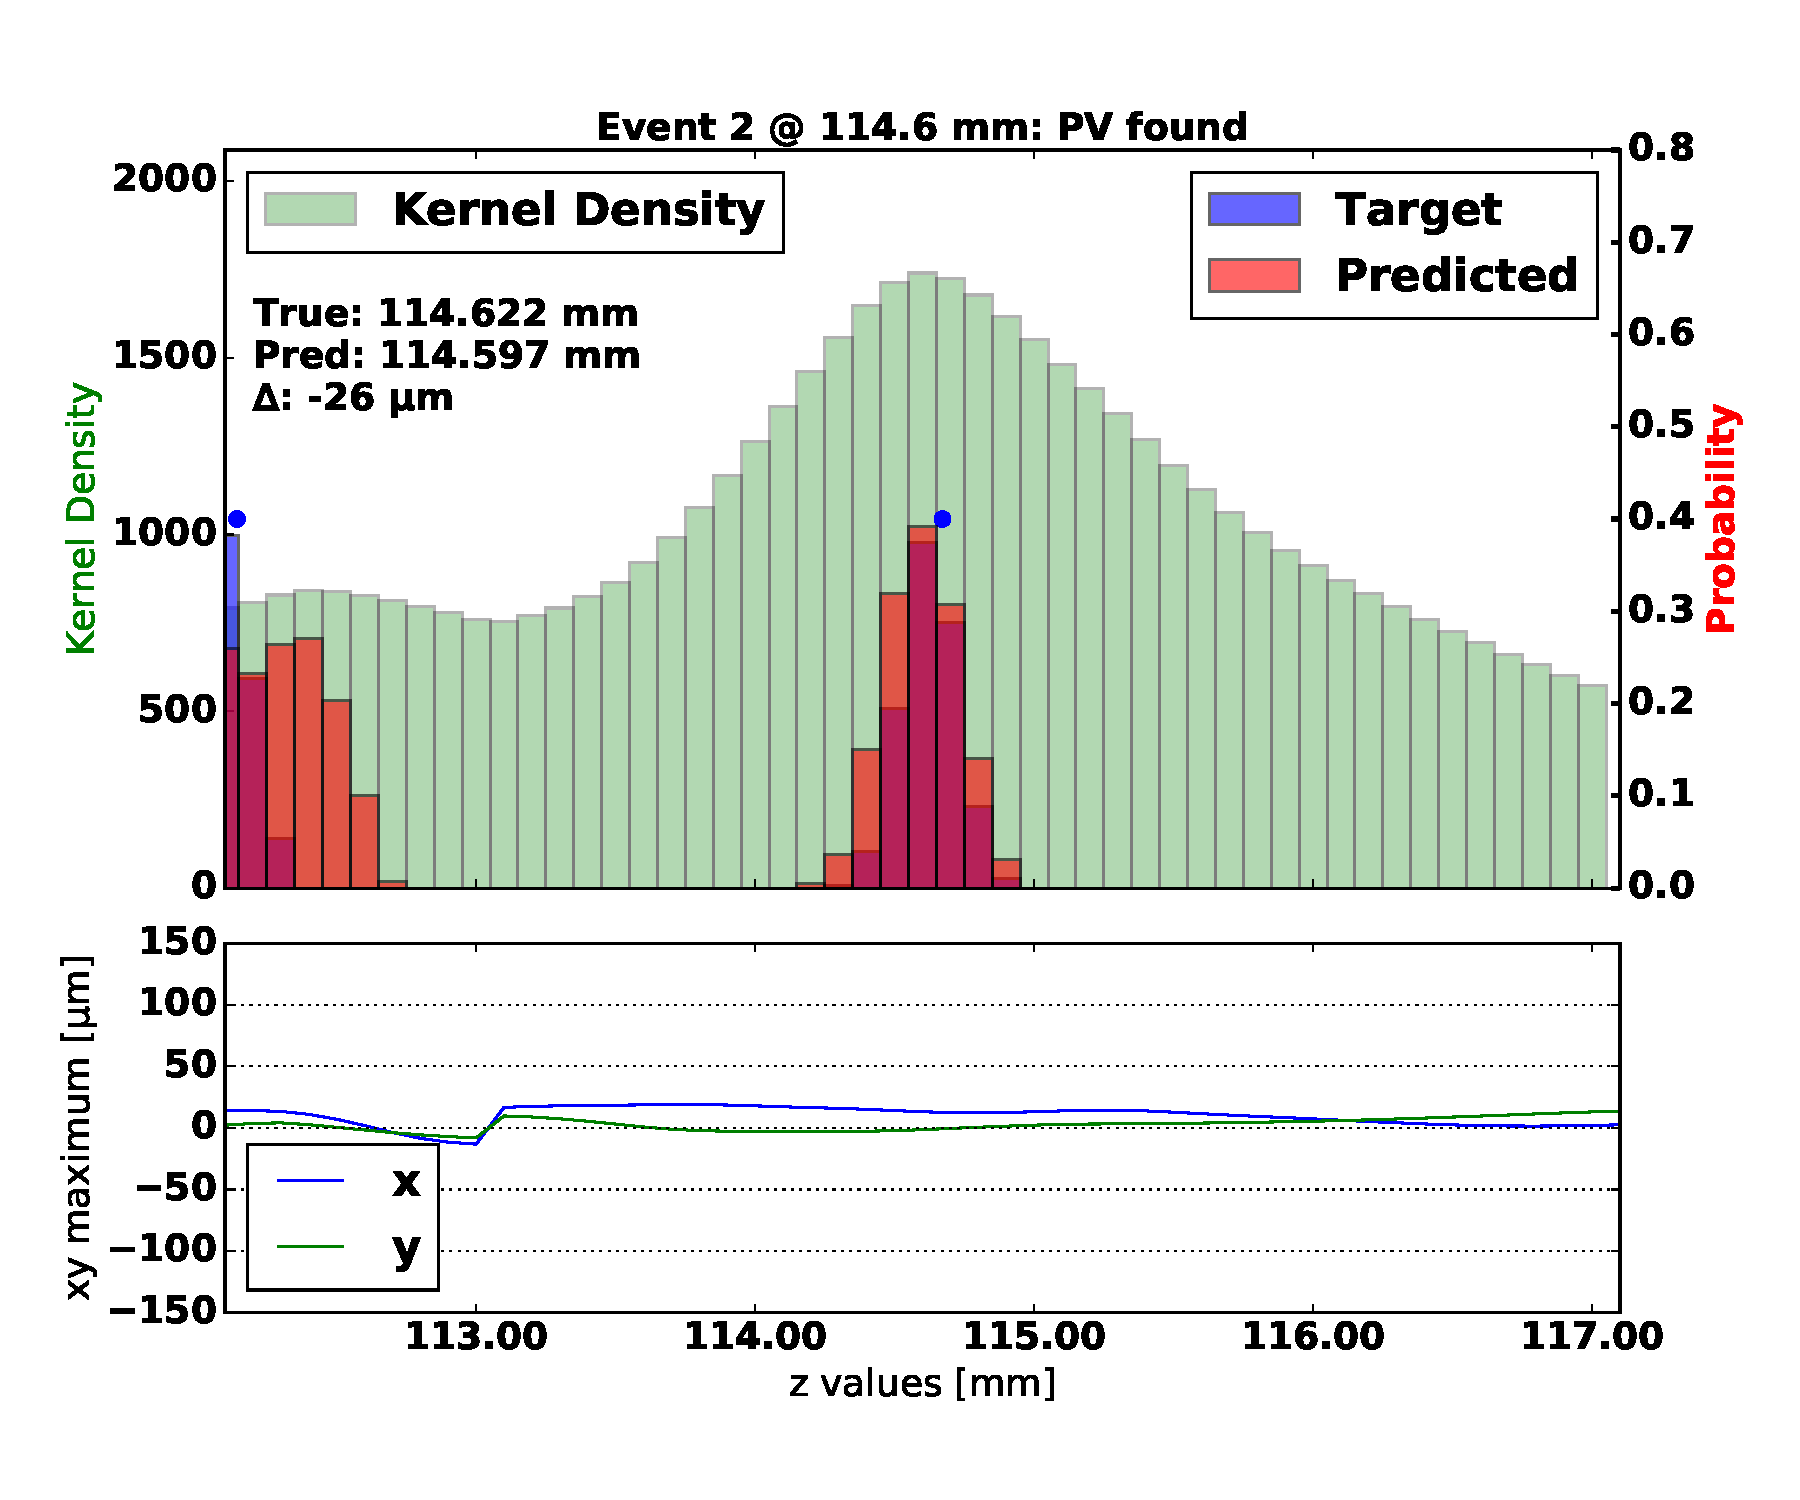
\includegraphics[width=1\textwidth, trim=60 0 60 0]{images/07Jan19_AltCNN4Layer_D35_sp_12.pdf}
 \end{center}
\end{columns}



\end{frame}
